\documentclass[10pt]{article}
\usepackage[margin=1in]{geometry}
\usepackage{amsmath,amssymb,amsthm}
\usepackage{graphicx}
\usepackage{booktabs}
\usepackage[colorlinks=true,linkcolor=blue,urlcolor=blue]{hyperref}
\usepackage{enumitem}
\usepackage{marginnote, easyReview}
\setlist{itemsep=1pt,topsep=2pt}
\newcommand{\ReLU}{\mathrm{ReLU}}
\newcommand{\Var}{\mathrm{Var}}
\newcommand{\Cov}{\mathrm{Cov}}
\newcommand{\E}{\mathbb{E}}
\newtheorem{fact}{Fact}

\title{The affine bulk-given-spike law in spiked ReLU networks:\\
exact one-layer analysis, the Bayes knee, and the spike-marginal recursion}
\author{One trained case --- \texttt{experiments/affine\_conditional\_layer1}}
\date{July 16--17, 2026}

\begin{document}
\maketitle

\begin{abstract}
\noindent
The binned / analytic K=2 predictors compress the bulk-given-spike conditional law of the
coordinate-spike model $M_\ell = W_\ell + e_1e_1^\top$ ($W\sim N(0,1/n)$, no training) to an
\emph{affine family} in the spike coordinate. Empirically this is excellent
\emph{post}-activation and mediocre \emph{pre}-activation at depth. This note collects the
mechanism, established in three steps with exact computations and MC at widths $128$--$4096$:
(1) after \emph{one} layer the post-activation conditional moments are affine with
$1-R^2\propto 1/n$ and closed-form constants;
(2) the failure at the next \emph{pre}-activation is a Bayes-posterior \textbf{knee} --- the
Tweedie correction $\omega^2\,\partial_a\log p(a)$ of a rectified (atom + branch) marginal seen
through a Gaussian channel --- which is $O(1)$ in $R^2$ terms and width-flat, rank-one across
coordinates, and predicted with zero shape parameters;
(3) depth propagation is governed by a \textbf{one-dimensional recursion on the spike marginal},
$p_{\ell+1} = \varphi_{\omega_\ell} * (c_\ell\ReLU + \mu_\ell)_{\#}\,p_\ell$, whose per-layer
scalar inputs are measurable, whose density prediction is accurate to $O(n^{-1/2})$ (dominated by
one scalar, $\kappa=w^\top m_1$; including it gives $O(n^{-1})$), and which shows the knee is a
damped fixed-point object ($q\approx 0.5$ per layer), not an accumulating one.
\end{abstract}

\section{Setup and notation}
Layers $Z^{(\ell+1)} = M_{\ell+1} H^{(\ell)}$, $H^{(\ell)}=\ReLU(Z^{(\ell)})$, $H^{(0)}=X\sim N(0,I_n)$,
$M_\ell = W_\ell + e_1e_1^\top$, $W_\ell\sim N(0,1/n)$ i.i.d. \emph{Spike} $A_\ell = Z^{(\ell)}_0$;
\emph{bulk} $Z^{(\ell)}_{1:}$. The surrogates assume, per layer, the affine family
\[
Z^{(\ell)}_{\mathrm{bulk}} \,\big|\, A_\ell = a \;\rightsquigarrow\;
N\!\big(m_0 + m_1 a,\; \Sigma_0 + \Sigma_1 a\big),
\]\marginpar{$Z$ is preactivation, so this assumption should only hold on post-activation}
and we measure its quality by the mass-weighted pooled $1-R^2$ of weighted-least-squares affine
fits of the true conditional moment curves (split-half debiased when the curves come from MC).
Throughout $\varphi,\Phi$ are the standard normal pdf/cdf, $\phi_0 = \varphi(0)=1/\sqrt{2\pi}$,
$\tau^2 = \Var(A_1) = \|M_1[0,:]\|^2 \approx 2$.

\section{One layer: affine to $O(1/n)$, exactly}
Conditional on $A_1 = s$, the bulk pre-activation is \emph{exactly} Gaussian
(joint Gaussianity of $Z^{(1)} = M_1X$):
\[
Z^{(1)}_{\mathrm{bulk}}\mid s \;\sim\; N(\beta s,\; C),\qquad
\beta = (M_1M_1^\top)_{\mathrm{bulk},0}/\tau^2 = O(n^{-1/2})\ \text{per coord},\quad C\ \text{const in }s .
\]
So pre-activation is trivially affine, and all post-activation curvature comes from the ReLU
moment maps $f(\mu,\sigma)=\E\,\ReLU N(\mu,\sigma^2)$, $g=\Var\,\ReLU N(\mu,\sigma^2)$, evaluated
at $\mu=\beta_i s$: analytic maps (the kink is convolved away by the $O(1)$ conditional noise
$\sigma_i$), probed on an interval of width $O(\beta_i\tau)=O(n^{-1/2})$. The affine model is the
tangent line; the residual is the quadratic Taylor term. With $f'(0)=\tfrac12$,
$f''(0)=\phi_0/\sigma$, $g'(0)=\sigma\phi_0$, $g''(0)=\tfrac12-\tfrac1\pi$, best-affine
fitting under the Gaussian mass of $s$ gives
\begin{equation}
1-R^2_{\mathrm{mean},i} \simeq \frac{2\phi_0^2\,\beta_i^2\tau^2}{\sigma_i^2},\qquad
1-R^2_{\mathrm{var},i} \simeq \Big(\frac{1/2-1/\pi}{\sigma_i\phi_0}\Big)^{\!2}\frac{\beta_i^2\tau^2}{2}
\qquad(\text{ratio } \approx 3.07),
\label{eq:taylor}
\end{equation}
both $\propto \beta_i^2 \propto 1/n$.

\begin{fact}[measured; widths 64--4096, 5 seeds, exact rectified-Gaussian conditional curves, no MC]
Pooled $1-R^2$: mean $1.87\times10^{-3}$, variance $6.05\times10^{-4}$, off-diagonal covariance
$1.07\times10^{-3}$ at $n=512$; $2.38\times10^{-4}$ / $7.7\times10^{-5}$ / $1.35\times10^{-4}$ at
$n=4096$; width exponents $-0.97,-0.96,-1.00$. Per-coordinate collapse onto \eqref{eq:taylor}
over nine decades. Fitted slope vector $=\Phi(0)\beta$ to machine precision
($\cos = 1-10^{-16}$); only $\cos\approx 1/\sqrt2$ of it lies along the naked column
$W_{[1:,0]}$ (the other half is row overlap $W_{\mathrm{bulk}}w_0^\top$). The conditional
variance is \emph{not} constant: it tilts with slope $2\phi_0\sigma_i \times$ the mean slope
($\approx 0.80$; measured $0.795$--$0.797$) --- a constant-$\Sigma$ model errs at $O(n^{-1/2})$,
the affine family at $O(1/n)$. The residual is a parabola in $s$: edge cells
($|s|\ge2.5\tau$) are $3.3\times$ worse, central ($|s|\le1.5\tau$) $3.2\times$ better, same
$1/n$ law; true failure needs $|\beta_i s|\sim\sigma_i$, i.e.\ a $\sim\!\sqrt{2n}$-sd spike
excursion. (Figs.~\ref{fig:l1}--\ref{fig:collapse}.)
\end{fact}

\begin{figure}[h]\centering
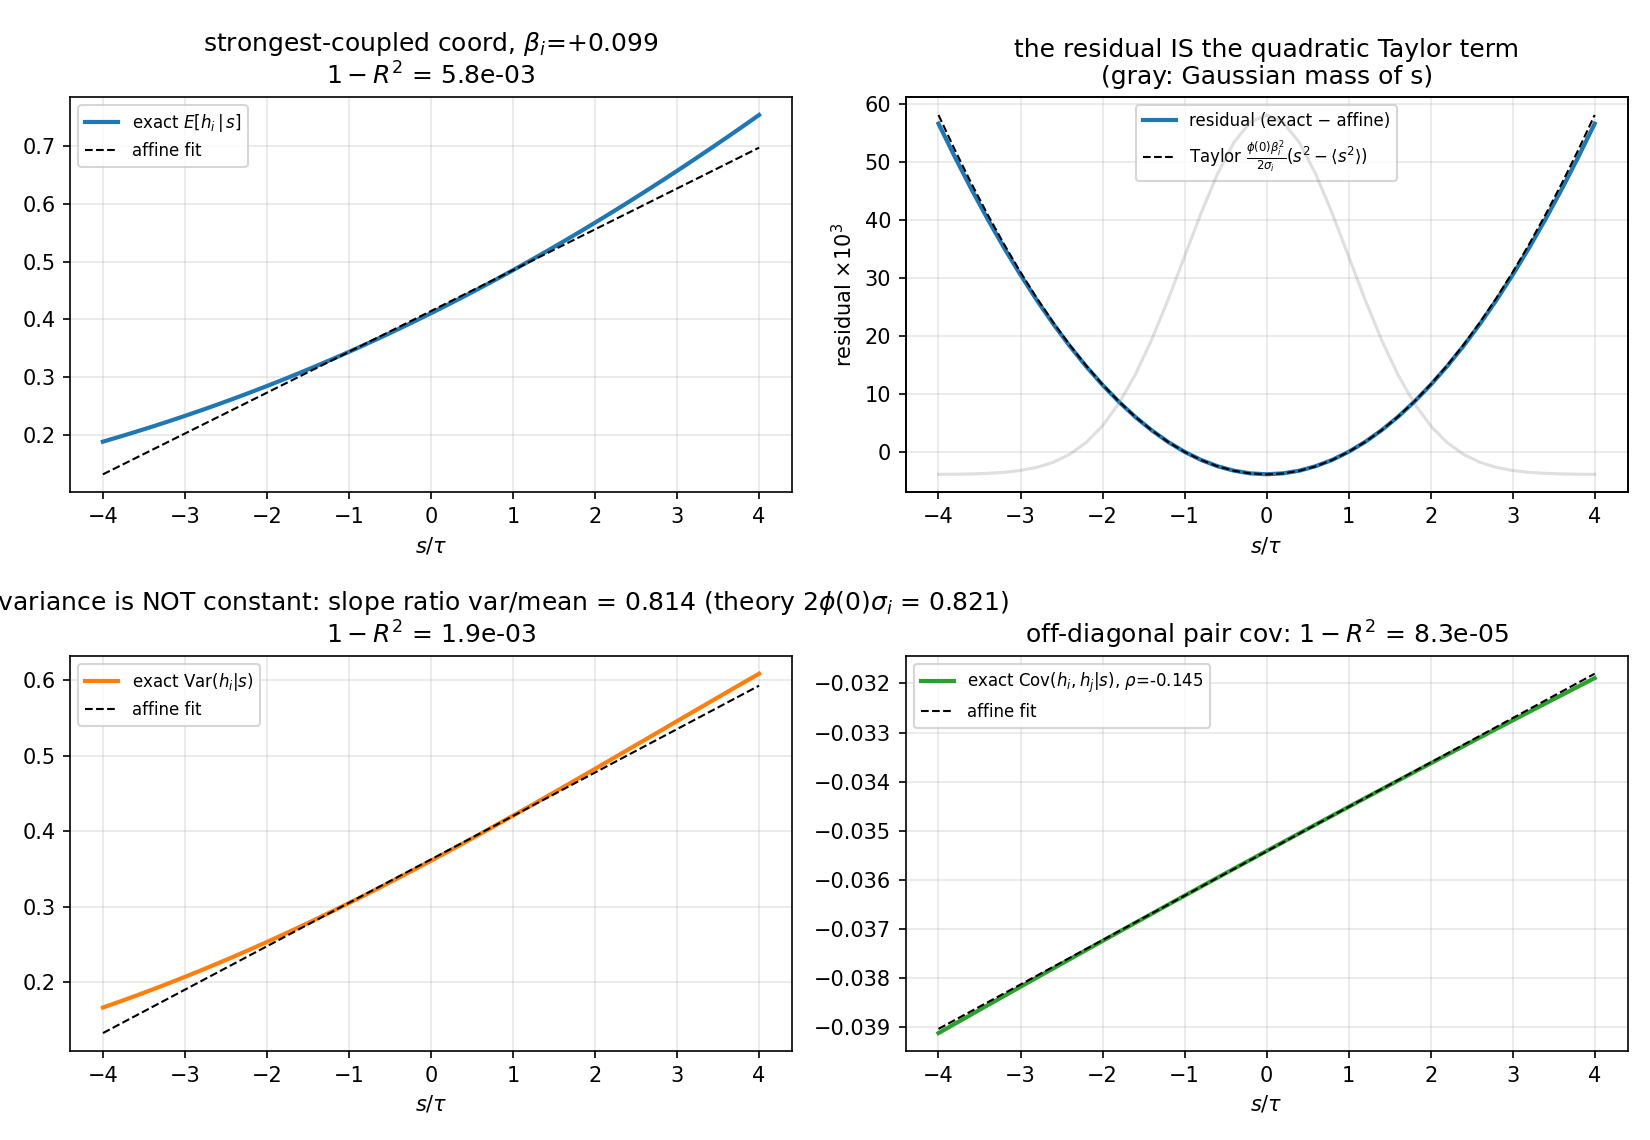
\includegraphics[width=.95\textwidth]{figs/F2_anatomy_n512.png}
\caption{Layer 1, $n=512$, strongest-coupled coordinate: the affine fit and its residual
$\equiv$ the quadratic Taylor term; the conditional variance tilts at $0.8\times$ the mean slope;
off-diagonal covariances are straightest.}
\label{fig:l1}
\end{figure}
\begin{figure}[h]\centering
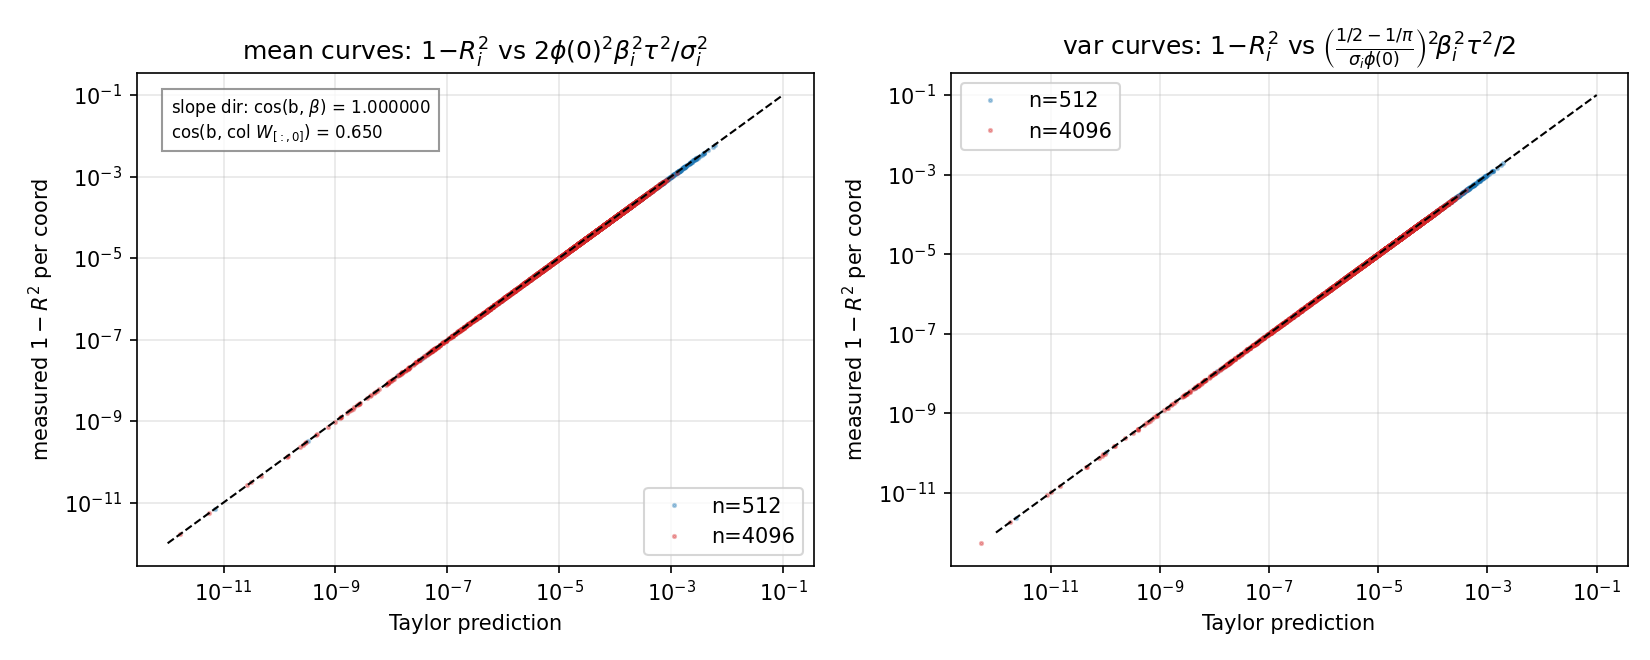
\includegraphics[width=.95\textwidth]{figs/F3_collapse.png}
\caption{Per-coordinate measured $1-R^2$ vs.\ the closed forms \eqref{eq:taylor}.}
\label{fig:collapse}
\end{figure}

\section{Why post-affine does not give the next pre-affine: the Bayes knee}
The next spike is, \emph{exactly},
\begin{equation}
A_{\ell+1} \;=\; c_\ell\,\ReLU(A_\ell) \;+\; \xi_\ell,\qquad
c_\ell = M_{\ell+1}[0,0]\approx 1,\qquad \xi_\ell = w_\ell^\top H^{(\ell)}_{\mathrm{bulk}},
\label{eq:channel}
\end{equation}
with $\xi_\ell \approx N(\mu_\ell,\omega_\ell^2)$ a fresh CLT sum ($\mu_\ell = w^\top m_0$ is an
$O(1)$ \emph{random-per-net} offset; $\omega_2^2\approx0.32$). Conditioning the new bulk on
$A_{\ell+1}=a$ routes through the posterior of the old variables: every coordinate obeys
\[
\E\big[Z^{(\ell+1)}_i \,\big|\, a\big] \;=\; \alpha_i + \rho_i a + \lambda_i\, g_{\ell+1}(a),
\qquad g_{\ell+1}(a) = \E\big[\ReLU(A_\ell)\,\big|\,A_{\ell+1}=a\big],
\]
one \emph{shared} profile $g$ with $O(n^{-1/2})$ coordinate amplitudes $\lambda_i$. Tweedie's
formula for the Gaussian channel \eqref{eq:channel} gives
\begin{equation}
c\,g(a) \;=\; a - \mu - \omega^2\,\partial_a \log p_{A_{\ell+1}}(a) :
\label{eq:tweedie}
\end{equation}
$g$ is affine iff the score is affine iff $A_{\ell+1}$ is Gaussian (Cram\'er) --- but
$\ReLU(A_\ell)$ has an atom plus a branch, so $g$ is a \textbf{knee}: a plateau (atom side),
a linear branch, and a crossover strip of width $\sim\omega$. Because $R^2$ is scale-free, the
$O(n^{-1/2})$ amplitude $\lambda_i$ divides out: pre-activation affine $1-R^2$ is $O(1)$ and
\emph{width-flat}. The conditional covariance picks up the rank-one term
$\tilde c\tilde c^\top \Var(A_\ell\,|\,a)$, whose coefficient is an S-curve with overshoot
($0\to0.50\to$ floor $(\tau^{-2}+\omega^{-2})^{-1}=0.40$) --- verified against MC along the
predicted direction at $n=2048$ (control direction flat).

\begin{fact}[measured]
Depth-2/3 nets, $n\in\{256,1024\}$, 1M samples, split-half debiased: layer-2 PRE
$1-R^2 = 0.156$--$0.168$, identical across widths; cross-half rank-one share $0.97$--$0.99$;
measured shared profile matches the zero-parameter knee at $\cos = 0.9986$--$0.9996$; amplitude
$\mathrm{rms}(\lambda)\sqrt n = 0.36$--$0.39$. The same knee measured at $n=2048$ (depth 2):
pooled PRE $0.155$ vs.\ $0.159$ predicted by the exact-in-surrogate quadrature.
(Fig.~\ref{fig:knee}.)
\end{fact}

\begin{figure}[h]\centering
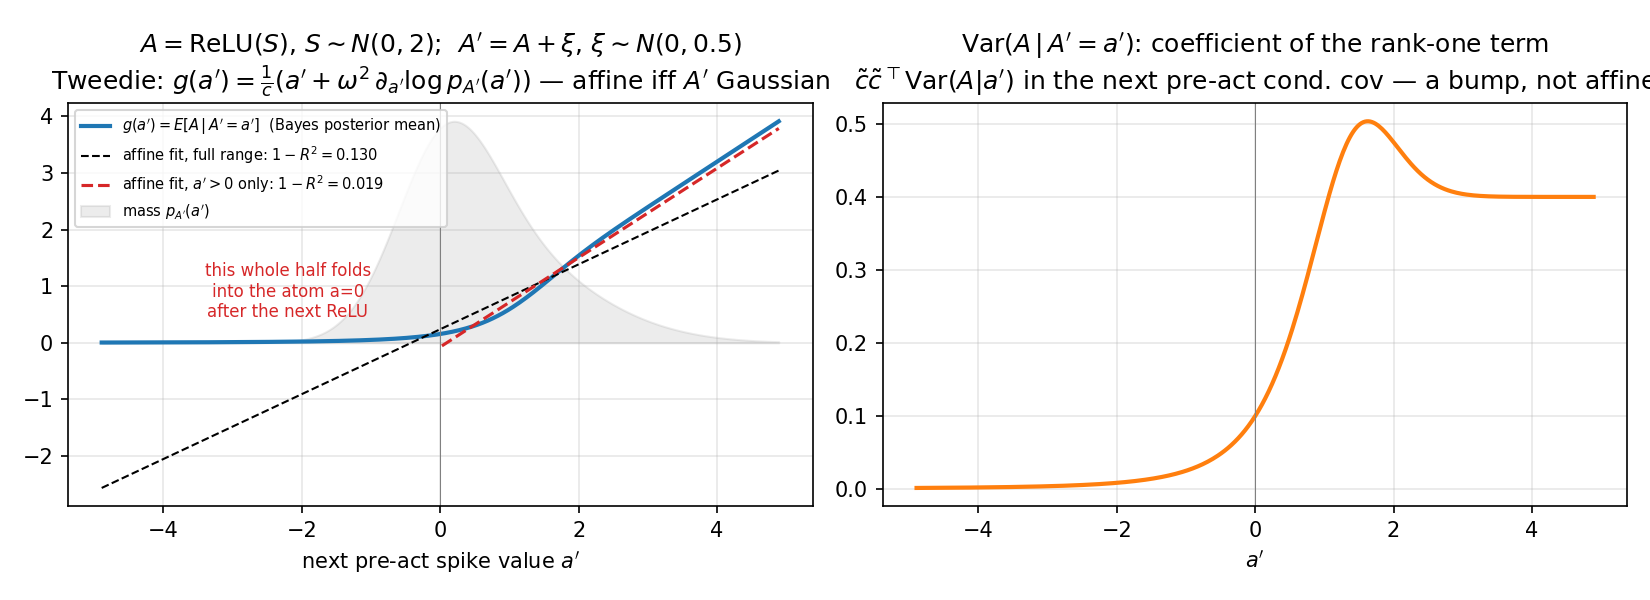
\includegraphics[width=.9\textwidth]{figs/bayes_knee.png}
\caption{The knee in a toy with the model's scales ($A=\ReLU(S)$, $S\sim N(0,2)$,
$A'=A+\xi$, $\omega^2=\tfrac12$): posterior mean $g$ (left) and posterior variance (right).
Affine fails at $1-R^2=0.130$ on the full range but only $0.019$ on $a'>0$ --- the half that
survives the next ReLU.}
\label{fig:knee}
\end{figure}

\paragraph{Why the ReLU restores affineness.}
The ReLU acts \emph{cell-wise} in the conditioning value: post moments at cell $a$ are smooth
rectified-Gaussian functions of pre moments at the same $a$, so it transports the knee with
factor $\Phi(0)=\tfrac12$ and adds only its own $O(1/n)$ curvature (Section~2). What changes is
the \emph{conditioning variable}: $a\mapsto\ReLU(a)$ folds the entire $a\le0$ half --- the
atom-dominated plateau and half the crossover --- into the single atom point, which the
positive-node affine fit does not see. Same curve, two verdicts: toy $0.130\to0.019$;
in-model POST (positive bins) $= 0.003$--$0.058$ at layers 2--3, i.e.\ $5$--$20\times$ below PRE,
with no depth trend.

\section{Depth: the spike-marginal recursion}
Iterating \eqref{eq:channel} marginally,
\begin{equation}
\boxed{\;p_{\ell+1}(a) \;=\; \int p_\ell(y)\;\varphi_{\omega_\ell}\!\big(a - c_\ell\ReLU(y) - \mu_\ell\big)\,dy,
\qquad p_1 = N(0,\tau^2),\;}
\label{eq:recursion}
\end{equation}
three measurable scalars per layer. At layer 2 it is closed-form: with
$u = a-\mu$, $b = c+\kappa$, $s_-^2=\kappa^2\tau^2+\omega^2$, $s_+^2=b^2\tau^2+\omega^2$
(and $\kappa = w^\top m_1$ the small linear pass-through),
\begin{equation}
p_2(a) \;=\; \underbrace{\tfrac{1}{s_-}\varphi\big(\tfrac{u}{s_-}\big)\,
\Phi\big(-\tfrac{\kappa\tau u}{\omega s_-}\big)}_{\text{smeared atom }(\to \frac12\varphi_\omega \text{ at }\kappa=0)}
\;+\;
\underbrace{\tfrac{1}{s_+}\varphi\big(\tfrac{u}{s_+}\big)\,
\Phi\big(\tfrac{b\tau u}{\omega s_+}\big)}_{\text{skew-normal branch}} ,
\label{eq:closedform}
\end{equation}
verified against quadrature to $\sim\!6\times10^{-6}$ TV and against 1M-sample MC to
TV $= 0.004$ (the sampling floor; Fig.~\ref{fig:cf}). For $\ell\ge3$, \eqref{eq:recursion} is the formula.

\begin{figure}[h]\centering
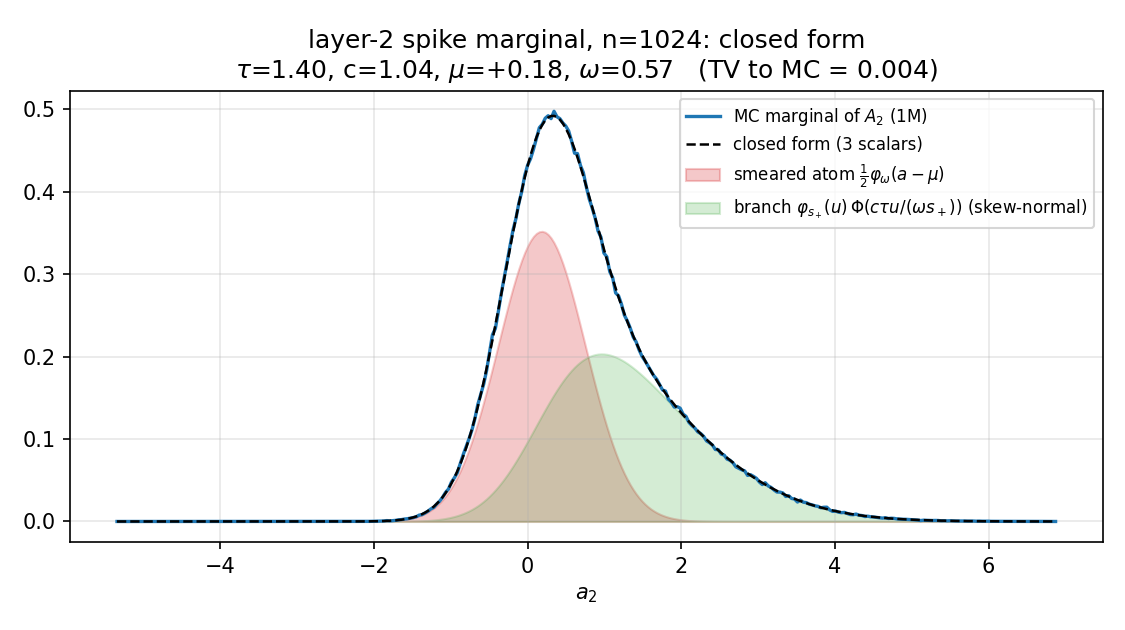
\includegraphics[width=.72\textwidth]{figs/F11_layer2_closed_form.png}
\caption{Layer-2 spike marginal at $n=1024$: closed form \eqref{eq:closedform} vs.\ MC.}
\label{fig:cf}
\end{figure}

\paragraph{Why the knee passes nicely through layers.}
(i) The fresh knee at every layer depends on the past \emph{only through the 1-d marginal}
\eqref{eq:tweedie}; it is irrelevant that $A_\ell$ is knee-contaminated and non-Gaussian.
(ii) Each layer re-smooths with a \emph{fresh} Gaussian $\xi_\ell$; for any $p = q*\varphi_\omega$
the posterior-variance identity $\Var(T|a) = \omega^2(1+\omega^2(\log p)'')\ge0$ caps the score
curvature at $-1/\omega^2$ --- the spoon can never sharpen beyond the channel noise, at any depth.
(iii) The \emph{old} knee propagates only as $Sg(a) = \E[g_\ell(A_\ell)\mid A_{\ell+1}=a]$ ---
smoothed by the posterior kernel (width $\approx$ the $\Var$ floor $\approx0.6$, the knee's own
feature size) and affine-projected: measured damping
$q = \|(I-\Pi)Sg\|/\|(I-\Pi)g\| = 0.34$--$0.75$ ($\approx0.5$ stationary), so nonaffine power
saturates geometrically instead of accumulating.

\begin{fact}[measured, depth 3]
Marginals: recursion vs.\ MC, TV $= 0.004$--$0.016$ at layers 2 \emph{and} 3 (all four nets).
Layer-3 PRE $1-R^2 = 0.057$--$0.172$: no systematic growth over layer 2; the seed scatter tracks
the random offsets $\mu_\ell$ (which decide where the knee sits in the mass), and the recursion
reproduces the seed ordering. Layer-3 profile $=$ recursion knee at $\cos = 0.984$--$0.999$;
rank-one share $0.88$--$0.96$, with the second component correlating with the predicted damped
layer-2 knee at $\cos = 0.43$--$0.59$. Under a stationary channel ($c=1,\mu=0,\omega^2$ fixed)
the fresh-knee $1-R^2$ \emph{relaxes} $0.103\to0.037$ over six layers with self-similar shape
($\cos\to0.997$). Caveat: this unnormalized net contracts bulk variance $\times\sim\tfrac13$
per layer, so $\omega_\ell^2$ shrinks ($0.32\to0.12$) --- very deep behavior is driven by that and
by $\mu$-drift, not by knee accumulation. (Figs.~\ref{fig:marg}--\ref{fig:depth}.)
\end{fact}

\begin{figure}[h]\centering
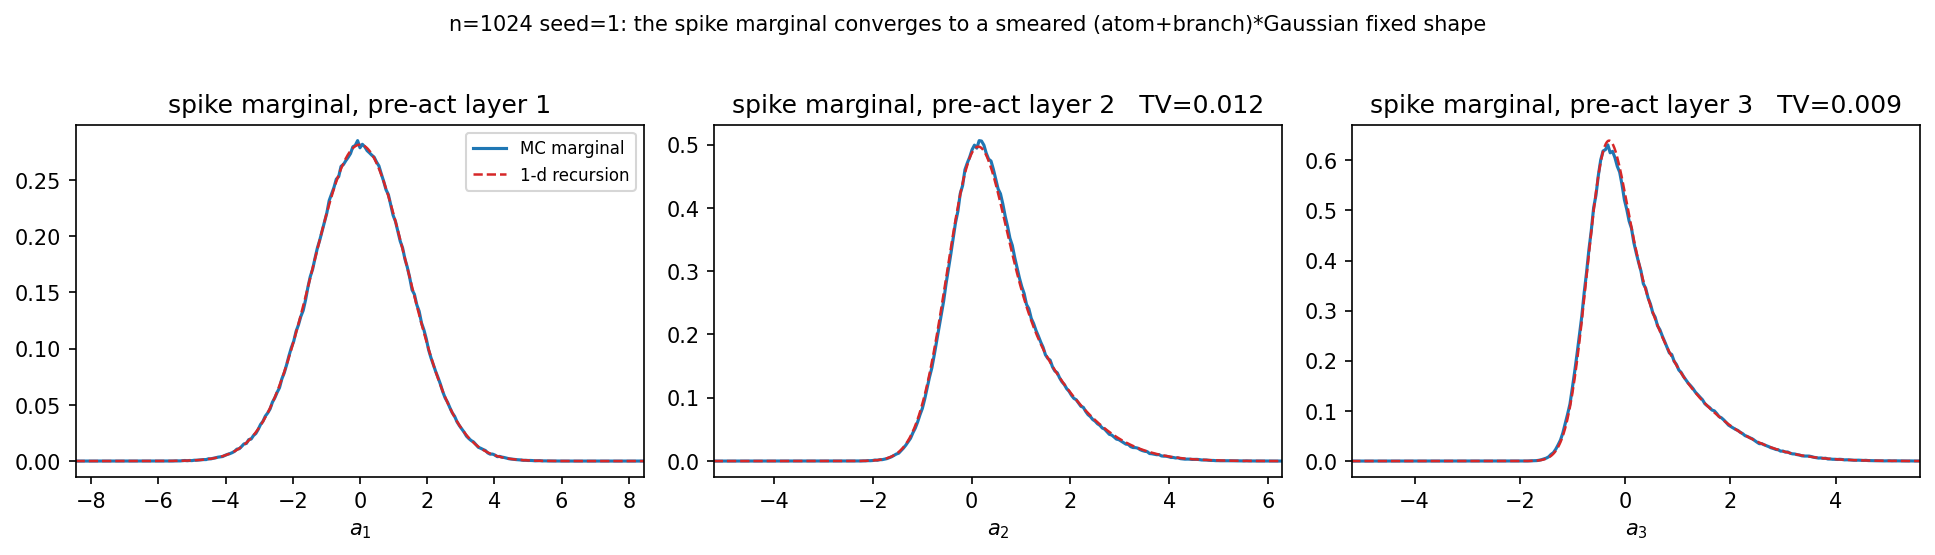
\includegraphics[width=.98\textwidth]{figs/F6_marginals_depth.png}
\caption{Spike marginals, layers 1--3 ($n=1024$): MC vs.\ recursion \eqref{eq:recursion}.}
\label{fig:marg}
\end{figure}
\begin{figure}[h]\centering
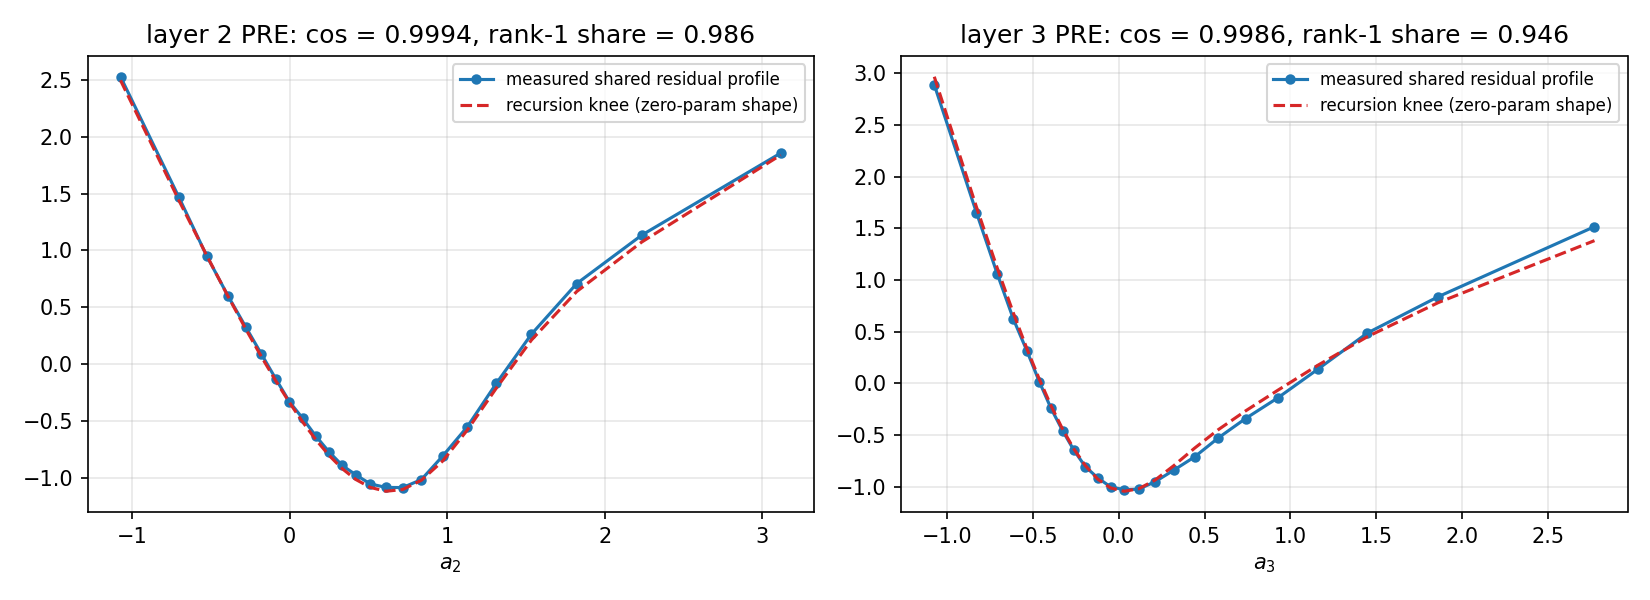
\includegraphics[width=.95\textwidth]{figs/F7_profiles_depth.png}
\caption{Measured shared affine-residual profiles at layers 2 and 3 vs.\ the zero-parameter
recursion knee.}
\label{fig:profiles}
\end{figure}
\begin{figure}[h]\centering
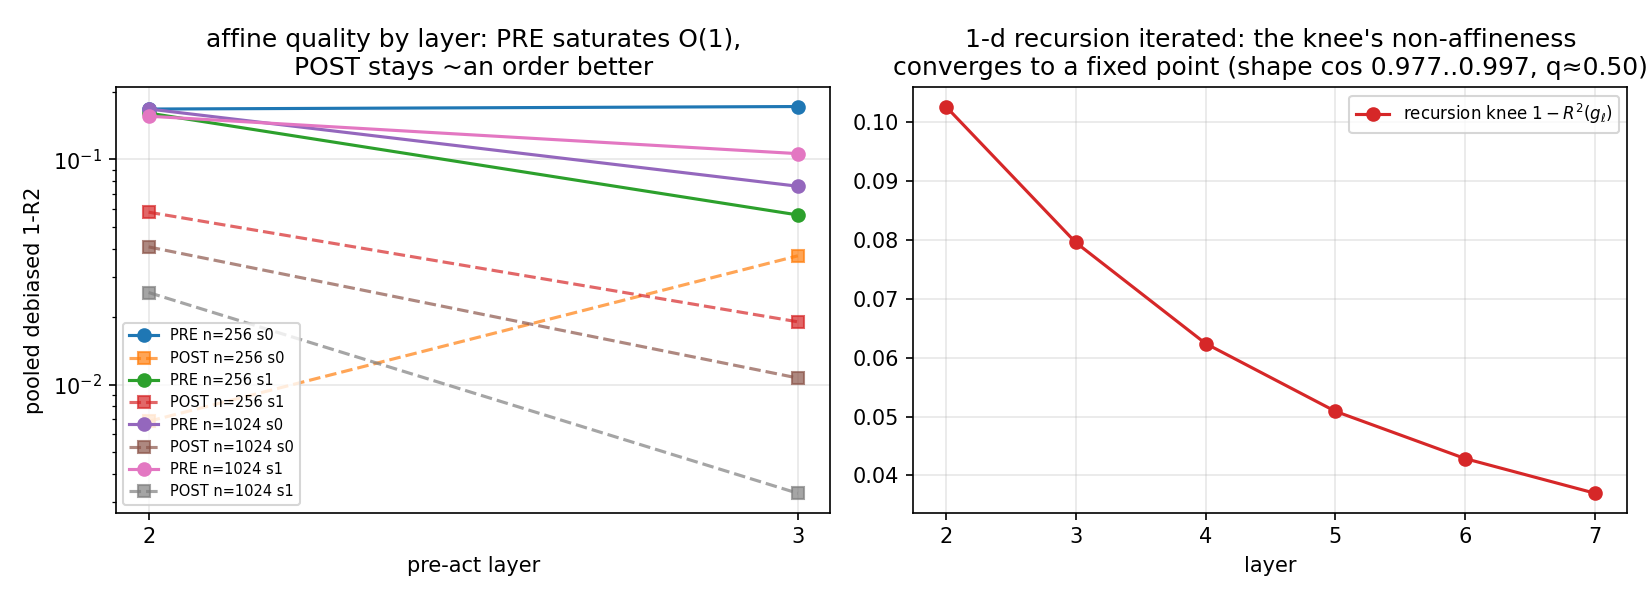
\includegraphics[width=.95\textwidth]{figs/F8_depth_degradation.png}
\caption{Left: PRE saturates at $O(1)$, POST stays an order better, both without depth growth.
Right: stationary-channel iteration of \eqref{eq:recursion}.}
\label{fig:depth}
\end{figure}

\section{Accuracy of the 1-d reduction: what is dropped and how it scales}
The recursion idealizes $\xi\,|\,A_\ell \sim N(\mu,\omega^2)$, independent of $A_\ell$. The exact
conditional channel is
\[
\xi \,\big|\, A_\ell = a \;\sim\;
N\Big(\mu + \underbrace{\kappa a}_{\kappa = w^\top m_1} + \underbrace{\lambda_w\, g_\ell(a)}_{\lambda_w = w^\top\lambda}
,\;\; \omega^2\big(1 + O(a/\sqrt n)\big)\Big) \;+\; \text{Edgeworth},
\]
so the bulk (``the other directions'') is \emph{not} small --- $\xi$ is $O(1)$ and is precisely
the smoothing --- but everything about it beyond $(\mu,\omega^2,\text{Gaussian})$ is
$O(n^{-1/2})$ or smaller:
\begin{center}
\begin{tabular}{llll}
\toprule
dropped term & size (theory) & measured & note\\
\midrule
mean tilt $\kappa = w^\top m_1$ & $N(0,\|m_1\|^2/n)$, $\|m_1\|=\sqrt{1/8}\approx0.354$ &
$|\kappa|\sqrt n \approx 0.35$ & dominant\\
old-knee leak $\lambda_w g_\ell(a)$ & $O(n^{-1/2})$ & inside $E[\xi|a]$ dev. & subdominant to $\kappa a$\\
variance tilt $\Var(\xi|a)/\omega^2 - 1$ & $O(n^{-1/2})$ & $\lesssim 0.03$ at $n{=}128$, noise-floor beyond & tiny\\
skewness of $\xi$ & $O(n^{-1})$ (random-sign $w$) & $0.08\to0.001$, $128\to2048$ & negligible\\
\bottomrule
\end{tabular}
\end{center}
Hence the predicted \emph{density} error amplitude is $O(n^{-1/2})$, i.e.\
$D^2 = \int(p-\hat p_{\rm rec})^2 \propto 1/n$, and including the single measured scalar
$\kappa$ should advance one order.

\begin{fact}[measured; cross-half-debiased $D^2$, widths 128--2048, 2 seeds]
Layer 3: $D^2 \propto n^{-1.00}$ (3-scalar recursion) and $\propto n^{-1.8}$ with the $\kappa$
tilt included. Layer 2 with $\kappa$: $D^2$ is zero within the 1M-sample noise floor
($|D^2|\lesssim10^{-5}$, TV $\approx 0.004$--$0.008$). Per seed, the 3-scalar error is
$\approx \kappa^2\Var(a)$ --- one scalar owns the leading error. (Fig.~\ref{fig:acc}.)
\end{fact}

\begin{figure}[h]\centering
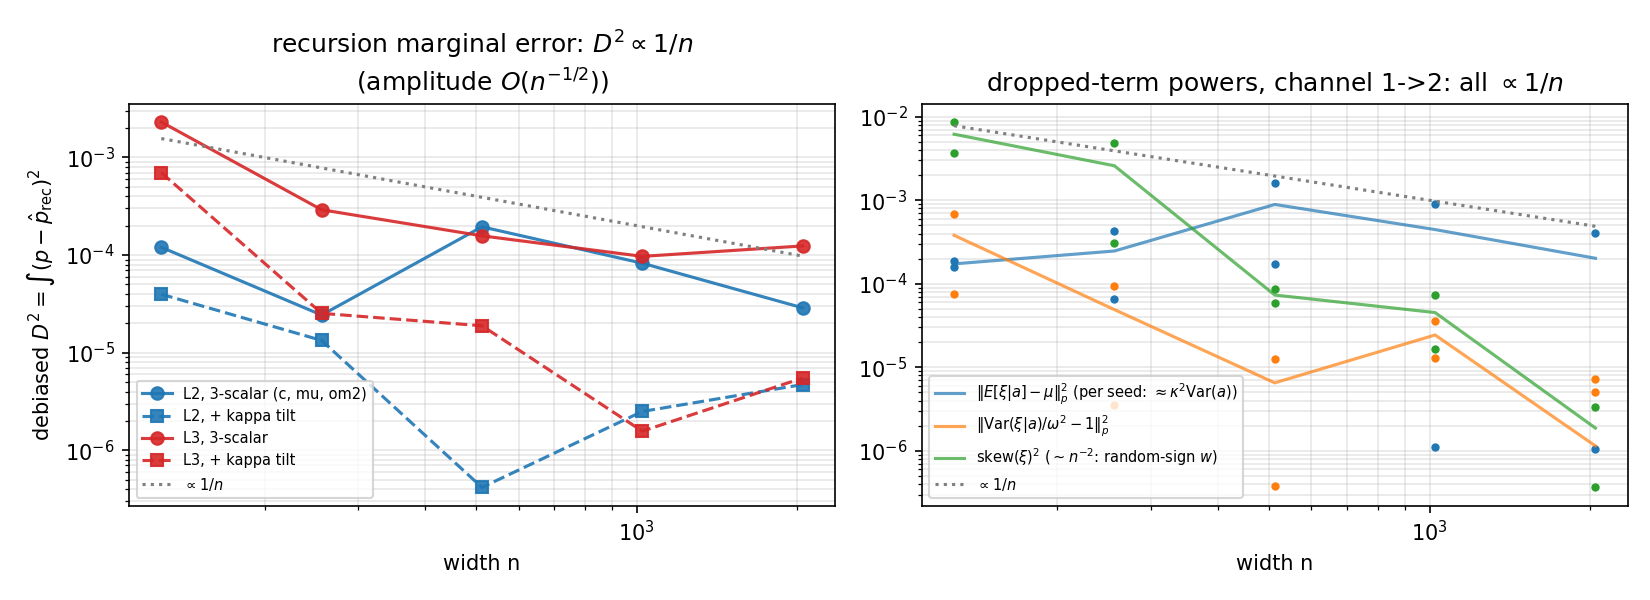
\includegraphics[width=.98\textwidth]{figs/F10_recursion_accuracy.png}
\caption{Left: debiased density error of the recursion vs.\ width. Right: dropped-term powers.}
\label{fig:acc}
\end{figure}

\section{Consequences and open ends}
\begin{itemize}
\item \textbf{Why affine-K2 predictors work:} the entire conditional structure is affine up to
(a) $O(1/n)$ within a layer (Section 2) and (b) one rank-one knee profile whose WLS-affine
projection is zero by construction ($g\perp\{1,a\}$), so it leaks into propagated \emph{moments}
only through the next ReLU's curvature, $O(1/n)$ per coordinate --- consistent with the observed
$n^{-2}$ MSE law and analytic$=$binned parity.
\item \textbf{Cheap upgrade:} augment the affine family with the single basis function
$g_\ell(a)$ from \eqref{eq:recursion}--\eqref{eq:tweedie} (rank-one knee correction; 3 scalars
per layer buy the profile).
\item \textbf{Discriminator:} this mechanism predicts deep POST $1-R^2$ floors at an
$n$-independent value set by the knee's positive shoulder rather than falling like $1/n$ ---
checkable against the \texttt{r2v2\_*} rows in \texttt{checkpoints/analytic\_kprop/r2/}.
\item \textbf{Caveat:} the unnormalized $W\sim N(0,1/n)$ net contracts bulk variance per layer;
with He-type $2/n$ scaling the channel scalars would be depth-stationary and the fixed-point
picture of Section 4 applies verbatim.
\end{itemize}

\paragraph{Artifacts.}
Notebook + builder: \texttt{experiments/affine\_conditional\_layer1/} (layer-1 exact study);
scripts \texttt{knee\_theory,knee\_mc,knee\_analysis} (layer-2 knee at scale),
\texttt{knee\_depth\_mc,knee\_depth\_analysis} (depth 2--3),
\texttt{knee\_channel\_mc,knee\_channel\_analysis} (channel structure, recursion accuracy).
Caches: \texttt{checkpoints/affine\_conditional\_layer1/} (\texttt{aff\_l1\_*},
\texttt{knee2\_*}, \texttt{knee3\_*}, \texttt{chanmc\_*}, \texttt{figs/}).
Shared kernel added: \texttt{Mecha\_preds/\_utils.py::exact\_relu\_covariance\_pairs}.

\end{document}
